\subsection{Opsætning af udviklings IDE til Arduino}

Dette afsnit har til formål at beskrive opsætningen af udviklings IDE'et til Arduino.
For at kunne gennemføre guiden skal AVR's Atmel Studio 6 og Arduino 1.0 eller højere være installeret på computeren. 

For at kunne compilere projekter til Arduino, kræves Arduino Core biblioteket i Atmel. Dette bibliotek bliver oprettet automatisk i Arduino IDE'et, men skal inkluderes i Atmel Studio.
Åben Arduino IDE'et og sæt flueben ved: Vis tydeligt output under kompilation.

\begin{figure}[H]
	\centering
	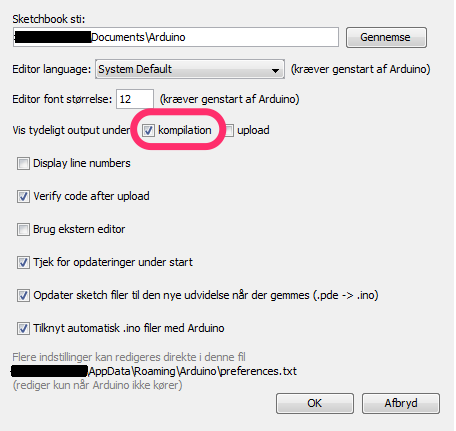
\includegraphics[width=0.5\textwidth]{Billeder/implementation/Howtoguide/Arduino_kompiler.png}
\end{figure}

I Arduino vælges et tilfældigt projekt, den rigtige arduino vælges under Værktøjer -> kort. Hvorefter skal koden kompileres. I vinduet i bunden vises en masse information, bla. stien for hvor core filen ligger. Stien ser ca. sådan ud, hvor det røde skiftes ud med dit brugernavn: 
\begin{figure}[H]
	\centering
	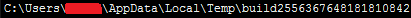
\includegraphics[width=0.85\textwidth]{Billeder/implementation/Howtoguide/core_sti.png}
\end{figure}
Inde i mappen ligger en core fil, denne fil skal kopieres over i Atmel Studio's workspace. Som standard ligger workspacet i "C:\textbackslash Users\textbackslash din bruger\textbackslash Documents\textbackslash Atmel Studio. 
Inde i Atmels workspace oprettes en mappe: "ArduinoCore" eller lignende. Core filen kopieres, lægges i mappen og navnet på filen ændres til libcore.
Ved opstart af Atmel, vælges hvilken type chip arduino bruger.

\textbf{Compiler opsætning} \\
For at kunne kompilere koden, skal de rette indstillinger til Atmel Studio vælges. 
Inde i Atmel vælges: Project -> Projektnavn properties:
Toolchain menuen vælges. I configuration vælges All Configurations.

\begin{figure}[H]
	\centering
	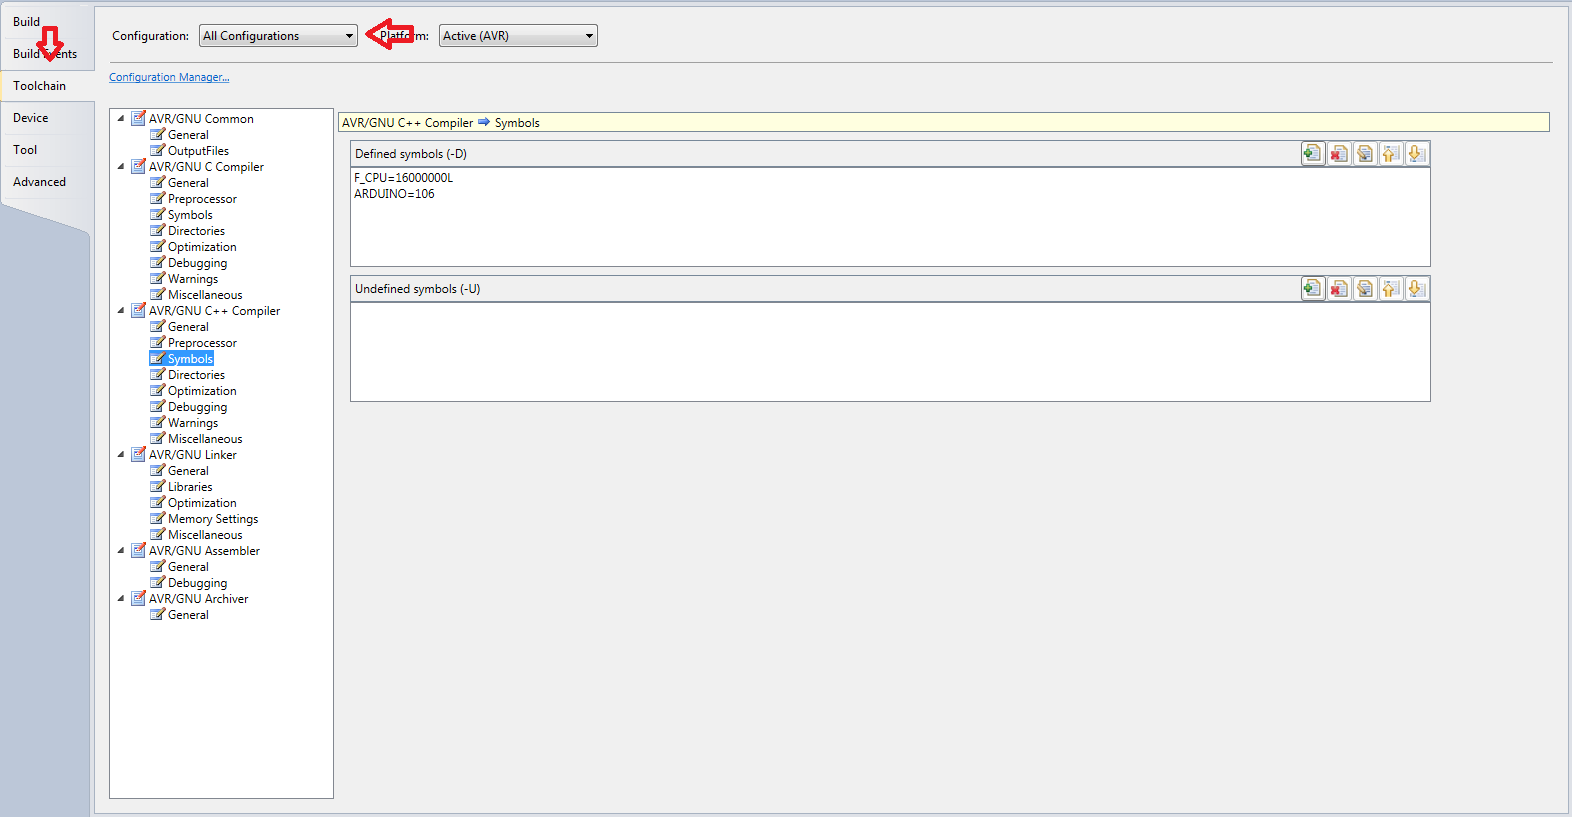
\includegraphics[width=0.85\textwidth]{Billeder/implementation/Howtoguide/atmel_toolchain.png}
\end{figure}

I menuen for GNU C++ compiler vælges Symbols. Her tilføjes clockfrekvens for arduino chippen og version af Arduino IDE.
For at tilføje clockfrekvens skrives fx: F\_CPU = 16000000L, hvis ens clockfrekvens er 16MHz.
Arduino IDE version skrives: ARDUINO=106, 106 for version 1.06. \\ \\

Næste trin er at opsætte Directories, det er stierne til de eksterne biblioteker til Atmel. Arduino har nogle biblioteker, som Atmel skal bruge, så dem skal der linkes til.
Bibliotekerne er henholdsvis Arduino.h og pins\_arduino.h
Stien til Arduino IDE'et er installations stien og resten af stien er som vist på billedet.
\begin{figure}[H]
	\centering
	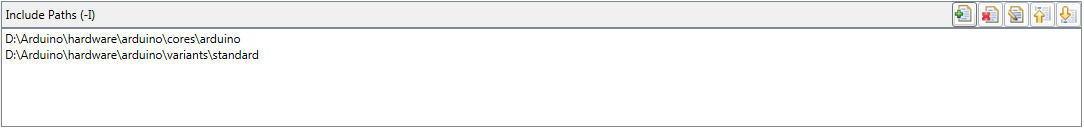
\includegraphics[width=1\textwidth]{Billeder/implementation/Howtoguide/atmel_directories.png}
\end{figure}

Gå til Optimization menuen under GNU C++ compiler og sæt flueben ved: Prepare functions for garbage collection (-ffunction-sections).\\ \\

I menuen for GNU Linker vælges Libraries. Her tilføjes core filen fra tidligere samt den sti den ligger i. En vigtig detalje er at core skal flyttes op over libm.
\begin{figure}[H]
	\centering
	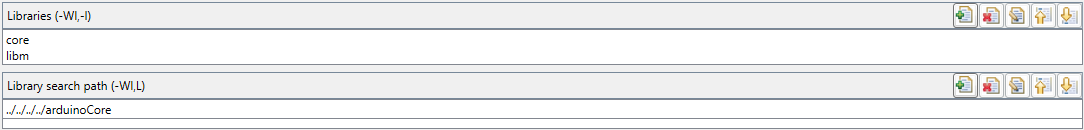
\includegraphics[width=1\textwidth]{Billeder/implementation/Howtoguide/atmel_linker.png}
\end{figure}

Atmel Studio er nu sat op til at fungere sammen med Arduino biblioteker. For at gøre brug af Arduino biblioteket tilføjes Arduino.h til projektet.

\subsubsection*{Eksterne bibliotekter til Atmel}

I Atmel og arduino findes der ikke standard JSon biblioteker, der kan håndtere JSon objekter. Det har derfor været nødvendigt at bruge et eksternt bibliotek, der kan håndtere disse JSon objekter.
Det anvendte bibliotek hedder aJson\footnote{https://github.com/interactive-matter/aJson} og er et frit tilgængeligt JSon bibliotek som er lavet til Arduino.


\subsubsection*{Filoversigt Drone}

Dette afsnit omhandler de forskellige filer og biblioteker der er anvendt i Atmel Studio. 


\begin{figure}[H]
	\centering
	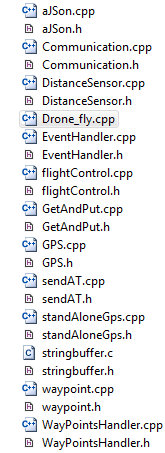
\includegraphics[width=0.25\textwidth]{Billeder/implementation/Howtoguide/atmel_filer.png}
\end{figure}

\textbf{aJSon}\\
JSon biblioteket håndterer sammen med stringbuffer biblioteket de JSon objekter der bruges af dronen. Der kan læses mere om JSon biblioteket her\footnote{https://github.com/interactive-matter/aJson} \\ \\
\textbf{Communication}\\
Communication klassen er den klasse der håndterer al kommunikation til dronen. Communication klassen er den øverste klasse i forhold til kommunikationen over 3G. \\ \\
\textbf{DistanceSensor}\\
Denne klasses funktionalitet er aflæsningen af sensorværdierne. \\ \\
\textbf{Drone\_fly}\\
Dette er selve mainen til systemet. Det er denne fil der håndterer alle andre klasser der anvendes i drone systemet. \\ \\
\textbf{EventHandler}\\
EventHandleren håndterer alle GET og PUT metoder der har med events at gøre. \\ \\
\textbf{FlightControl}\\
FlightControl klassen styrer selve dronen. Den får input fra både Flight Control boarded og 3G/GPS shieldet og udregner bl.a. orientering. \\ \\
\textbf{GetAndPut}\\
GetAndPut klassen er den klasse der er mest hardware nær i forhold til kommunikationen over 3G. Det er denne klasse der kontrollerer hvilken GET og PUT requests der skal sendes og til hvilken server. \\ \\ 
\textbf{GPS}\\
Denne klasse er en abstrakt klasse, som kun indeholder virtuelle metoder. Det gør at andre klasser der bruger denne abstrakte klasse, som minimum skal implementere de virtuelle metoder. \\ \\
\textbf{sendAT}\\
sendAT er taget med for at kunne sende AT kommandoer til 3G/GPS shieldet. \\ \\
\textbf{standAloneGps}\\
standAloneGps håndterer den valgte GPS og de metoder der skal bruges for at hente GPS koordinater. \\ \\
\textbf{waypoint}\\
Waypoint klassen håndterer det data WayPointsHandleren får.\\ \\
\textbf{WayPointsHandler}\\
WayPointsHandleren håndterer alle GET og PUT metoder der har med  waypoints at gøre. \\ \\





\subsection{Opsætning af serial programmerings link}

For at kunne uploade kode til en arduino, skal der anvendes et andet program.
Megunolink lite er et program med en brugergrænseflade der kan anvendes til at sende og modtage seriel data fra en arduino.\\
MegunoLink lite hentes her\footnote{http://www.megunolink.com/megunolink-lite/megunolink-lite-plotting-tool/}.

MegunoLink skal sættes op til at uploade til den korrekte Arduino. 

I configuration benyttes "use custom path" og ved AVRDude stien linkes til stien med AVRDude til arduino og configurationens stien. 

\begin{figure}[H]
	\centering
	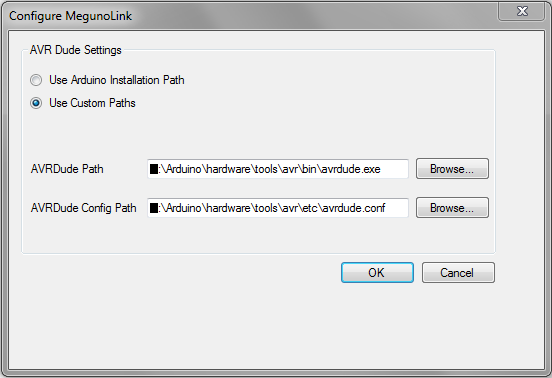
\includegraphics[width=0.7\textwidth]{Billeder/implementation/Howtoguide/megunolink_config.png}
\end{figure}

For at kunne uploade, skal MegunoLink vide hvor hex filen ligger, denne vælges i edit project properties også stien for det valgte projekt.
I dropdown menuen vælges den arduino der skal bruges til projektet.
\begin{figure}[H]
	\centering
	
\includegraphics[width=1\textwidth]{Billeder/implementation/Howtoguide/meguno_bar.png}
\end{figure}






